\section{Zielsetzung}
In diesem Versuch soll der Phasenübergang von Wasser von flüssig zu gasförmig untersucht werden.
Dafür soll die Verdampfungswärme des Wassers in Abhängigkeit der Temperatur ermittelt und insbesondere eine Dampfdruckkurve
erstellt werden.

\section{Theorie}
Allgemein kann Wasser die Phasen fest, flüssig und gasförmig annehmen. Diese Phasen lassen sich in einem Zustandsdiagramm (s. Abbildung \ref{fig:theorie1})
darstellen. In dem Zustandsdiagramm ist der Druck $p$ gegen die Temperatur $T$ aufgetragen und mit Hilfe dreier Kurven lassen sich Bereiche abgrenzen, die 
die Phasen definieren. In den durch die Kurven abgegrenzten Arealen hat das System die zwei Freiheitsgrade $p$ und $T$.\\
Sobald sich der Punkt $(T{,}\,p)$ einer der Kurven nähert erreicht man Zustände in denen zwei Phasen koexistieren. Dies ist für die Punkte TP. und K.P. der Fall, die
auch den Anfangs- und Endpunkt der Dampfdruckkurve charakterisieren.
\label{sec:Theorie}
\begin{figure}
    \centering
    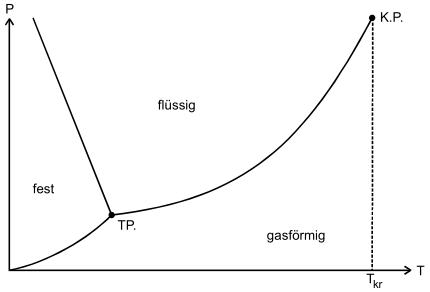
\includegraphics{Theorie1.png}
    \caption{qualitatives Zustandsdiagramm des Wassers \cite{sample}}
    \label{fig:theorie1}
\end{figure}
Auf der Dampfdruckkurve hat das System nur noch einen Freiheitsgrad, da $p$ und $T$ nicht mehr beliebig wählbar sind.

\cite{sample}
